\paragraph{Casing}

When the components are tested and fully operational in laboratory conditions, they will need to be packaged into the casing. The following
characteristics need to be considered when determining which case is best suited for this application:

\begin{itemize}
\item {Quality} 
\item {Size/Orientation}
\item {Heat Dissipation} 
\item {Cost} 
\item {External Connectors}
\end{itemize}


When the package is mounted onto the Newport Bridge, it will be exposed to harsh weather conditions: wind, precipitation, extreme temperatures,
etc. Therefore, it is essential to utilize a case that can withstand these conditions. O-rings are necessary to prevent water from leaking into
the case through the seal of the lid. This water can easily damage the electrical components within the package. The case will also have to be able to
withstand possible extreme temperatures. If the case cannot withstand the possible cold temperatures it will be exposed to without cracking, water can
leak into the package and destroy the equipment. High temperatures can cause the case to melt/deform which may possibly affect the retrieved data. 

It will be important to choose a case that not only large enough that can house all of the equipment but also fits the equipment in a manner that it can
be neatly organized and arranged. This allows for a quicker and more efficient package assembly. This also allows for a quicker examination of the
set-up in case an error occurs. To account for this, the orientation of the case is important. For example, a top-loading bucket (such as the Pelican
1430 seen below) would not be practical because it would be very difficult to access the components once the package is assembled and mounted.  



Electrical devices are only operational within a specific temperature range where if the maximum or minimum temperatures are exceeded, the component may
not fully function or even fail completely. To determine if the SHM system will fail due to extreme temperatures, the temperature inside the case must
be calculated. The enclosed volume has two major sources of temperature flux: the external temperature and the work done by the system. The first step
will be to calculate the heat transferred from the electrical components using the equation:

\begin{equation}
q(eq) = P(eq)*K_1*K_2
\end{equation}

where $q(eq)$ is the heat transferred from electrical equipment in Watts (W), $P(eq)$ is the electrical power consumption (W), $K_1$ is the load
coefficient, and $K_2$ is the running time coefficient. This value will then be inserted into the 1-D heat transfer equation:

\begin{equation}
q=k*A*\frac{\Delta T}{dx}
\end{equation}

where $q$ is the heat due to the electrical components, $k$ is the thermal conductivity of the material, $A$ is the area of which heat is being transfered
through, $\Delta T$ is the change in temperature, and $dx$ is the thickness of material. This equation will need to be computed for the heat transfer
through each of the casing walls, as well as the corners of the case, then averaged using the equation: 

$$q_t = sqrt((q_x)^2+(q_y)^2+(q_z)^2+(q_c)^2)$$

where $q_c$ is the heat transfer through the corners of the case. The resulting value will then be used with the maximum expected temperatures based on
temperature history data, such as that provided by NOAA, to determine the maximum temperature at which the system will still operate. If the resulting
temperature is higher than the lowest maximum operating temperature out of all the components, the system may fail, and that case may not be the best
option. That same principal can be applied to when the system is not generating any heat with respect to the minimum expected external temperature and
highest minimum operational temperature of the components. Ideally, once the package is fully modeled, the heat transfer equation can be more
thoroughly and accurately calculated by accounting for the spatial orientation between the components and the interior walls of the case. However,
if the components are mounted in place via foam cutouts, the heat dissipation between the components and the foam must first be calculated, and then
the heat transfer between the foam and the interior walls will then be calculated.

\paragraph{External Connectors} 
Several external connectors will need to be installed on the case walls for the full functionality of the SHM system. These ports need to be waterproof
with tight seals to prevent water from entering the case or external connections. The waterproof connections will require secure mating mechanisms, such
as locking and screwing mechanisms shown in Figure~\ref{fig:BowChicaWowWow}, to ensure that that the male ends will not become unplugged thus allowing
water to enter the connection and damage it. Each connector will also require a bulkhead cap to cover and protect against water damage if the
connector is not in use. These external connections are going to be implemented for a variety of sub-systems within the SHM package: energy
scavenging devices, BeagleBone Black, strain gauge, GPS, and XBee.
\begin{figure}[h]
\centering
\includegraphics[width=0.3\textwidth]{Wiley_MatingStyle.JPG}
\caption{\label{fig:BowChicaWowWow} Example Mating Mechanisms}
\end{figure}

Power connectors will be used to connect the wind turbine and solar panels to the package. These connectors must be rated for a high enough current to
match the power source. For example, since the wind turbine is rated up to 27A, the power connector should have a current rating that is similar enough
that there will not be damage done to the port due to the excess current. Each power connection will have a female port installed on the side of the
case and a corresponding male jack will need to be installed at the end of the power input. If multiple solar panels are utilized, either the power
inputs need to be put into parallel in one wire to input all the energy through one connection or a connector needs to be installed for as many panels
are used. 

A USB 2.0A port will be installed to access the BBB without having to open the package via a flash drive. This type of USB port was chosen to match the
same type of connection specified from the BBB data sheet. The connector gender of this port needs to be female to plug a USB chord to access the BBB,
such as the one seen in Figure \ref{fig:USB}. 
\begin{figure}[h]
\centering
\includegraphics[width=0.3\textwidth]{Wiley_USB2Aport.JPG}
\caption{\label{fig:USB} USB 2.0A External Connector (LTWUA-20AMFM-SL7A) from Ampehnol LTW}
\end{figure}

There are a few different types of connectors that can be used to attach the leads of the strain gauge to the package. Unlike the rest of the
connections, the strain gauge leads do not require a certain type of connection terminal. One option is to attach the leads to either a category 5 (CAT
5) or CAT5e shielded Ethernet cable and install an external connection for such a cable as seen in Figure~\ref{fig:CAT5}. Category type cables are
designed for high signal integrity to achieve performance standards set by organizations (such as IEEE) (citation). \todo{this citation was exported
form Google as a .BibTex file.}. This type of cable will ensure that the signals are relayed to the ADC reliably. A shielded cable is desired to
ensure that the sensitive signal being sent from the strain gauge to the ADC does not get disturbed by noise. 
\begin{figure}[h]
\centering
\includegraphics[width=0.3\textwidth]{Wiley_CAT5EthernetConnection.JPG}
\caption{\label{fig:CAT5} Shielded Ethernet External Connector (RJ45-5EWTP-QR-PCB) from Video Production Inc}
\end{figure}

An alternative method is through the use of waterproof cable glands (see Figure~\ref{fig:Cable Gland}. The leads would be attached to a cable, preferably
shielded, and fed through the gland which would then be sealed. The proper gland must be matched up to the outer diameter of the cable otherwise the
gland will not be water tight. These are advantageous because not only do individual cable glands work with a range of cable thicknesses, but different
gland diameter ranges can be found. 
\begin{figure}[ht]
\centering
\includegraphics[width=0.7\textwidth]{Wiley_CableGland.JPG}
\caption{\label{fig:Cable Gland} Cable Gland (CB-GD-5000045) from AA Power Corp}
\end{figure}


The GPS antenna attaches to the GPS via the use of a coaxial MCX connection. Two viable options for connecting the antenna are to implement a waterproof
MCX connector or a cable gland. Implementing a waterproof MCX connector on the package may be difficult because MCX connectors are very small as evident
by Figure \ref{fig:MCX}. If one of these connectors is able to implemented, it will be essential to choose the proper impedance level of the
connector. The other option is to implement a cable gland, such as the alternative option for the strain gauge above in Figure~\ref{fig:Cable Gland},
to run a wire through the case wall between the antenna and the GPS. The antenna would then need to be fastened to the outside of the case or another
substrate to prevent it from freely swinging around. 
\begin{figure}[ht]
\centering
\includegraphics[width=0.7\textwidth]{Wiley_MCX.JPG}
\caption{\label{fig:MCX} MCX Jack-to-Jack Adapter (252171) from Aamphenol Connex with Size Reference}
\end{figure}


The final component that requires and external connector is the XBee.The XBee antenna attaches to the device itself via the use of an SMA connection. A
waterproof coaxial connector, like the one shown in Figure~\ref{fig:SMA}, can be implemented as the external connector as well as a cable gland. 
Similarly to the MCX connector, the SMA connector is also small which may make utilizing one of these difficult. However, if a cable gland is used, the
antenna may need to be mounted to the case or other substrate to prevent it from freely swinging around as is the case with the GPS.
\begin{figure}[ht]
\centering
\includegraphics[width=0.7\textwidth]{Wiley_SMAconnector.JPG}
\caption{\label{fig:SMA} Waterproof SMA Bulkhead Connector (9153-7553-002) from Applied Engineering Products with Size Reference}
\end{figure}



\paragraph {Case Selection} Attempts were made to try to obtain the actual thermal conductivity coefficients for different cases, but unfortunately proper
data was never able to be retrieved due to lack of information from retailers. Since the general material of the considered cases is known, an
estimation of the thermal conductivity coefficient was made because studies have been performed to determine $k$ values for different materials. 
However, continued efforts to obtain this information may supply data to more accurately calculate the heat transfer through the casing walls. The
thickness of each case will need to be considered for two reasons. The first reason is that the thickness of the case affects heat transfer. Thicker
cases will allow for less heat transfer through the casing walls. The other is that the thickness of the casing wall affects whether or not certain
external connectors can be implemented. If the case is too thick, many MCX and SMA connectors may not be able to be installed because the case may
be thicker than the connector is long. When comparing costs, it should be later noted of any accessories, whether they are necessary or
convenient, that can and will be purchased. For example, the Ultra-case 613 by UW Kinetics charges another \$6.99 for the required O-ring to
water proof an already expensive case, so this may not be the most suitable case for this application. For a look at the a comparison of nominal
characteristics of the cases that were considered, see \ref{sec:Appendix Case Comparison}.

\paragraph{Assembly Layout}


When the package is ready to be assembled, the interior layout of the components needs to be determined. A few factors will need to be considered. 
The first is the location of external connectors. As stated above, the thickness of the case will affect what type of connectors may need to used. 
An example of this is shown in Figure \ref{fig:Assembly} which is a potential 2-D assembly layout using a Pelican 1400 model case. If an SMA
connector is used instead of a cable gland, it would need to be installed on the shorter wall since the case does not have a uniform thickness and
that wall is the only one thin enough out of the two to install such a connector. It would not make to sense to install the connectors through
the lid either because opening the case may place too much tension on the wires causing damage. 

\begin{figure}[h]
\centering
\includegraphics[width=1\textwidth]{Wiley_2DAssemblyLayout.jpg}
\caption{\label{fig:Assembly} Potential Layout of a Pelican 1400 Model Case}
\end{figure}

It will also be important to orient the breadboard in a manner that the accelerometer measures data in the intended direction as if it was mounted. 
Otherwise, it will need to be understood that the data measured on each axis during lab trials will not be measured along the same axes in the field and
will need to be accounted for while analyzing the data. 

\paragraph{Package Location}

\indent Figure \ref{fig:PackageLocation} is an Abaqus visualization of the Newport Bridge with the proposed location for the sensor package to be mounted.
As shown in the figure, the center of the bridge is the best location for the sensor package. This is because the greatest amplitude of displacement will
occur during the first mode of vibration at the middle of the bridge. Mounting the sensor package to the bridge must be done without damaging the
structure in any way. The sensor package must also be capable of being moved easily. Most importantly, the package must be secured without any of its
own motion so that the sensors can recognize the movement of the bridge and not the movement of the package itself. 

The most economical way of securing the sensor package to the bridge is to use powerful magnets. Neodymium Magnets are strong magnets that work well in
all environments and resist demagnetization. One negative aspect of magnets is that they can be prone to corrosion if a protective coating is not
properly applied. There is also a concern that the magnetic field can disrupt the electronics within the case. However, these issues can be prevented if
the correct precautions are taken. These magnets come in many shapes and sizes, as shown in Figure \ref{fig:Mounting Magnet}, and can be purchased with
pre-fabricated holes for screws to attach the magnets to the exterior of the case. The magnets in figure \ref{fig:Mounting Magnet} are the MMR-A-XC
model of magnets from KJMagnetics.com. This magnet is hardly larger than a penny, yet it can easily be screwed into the sensor package and has a
holding force of 54.14 pounds. With two of these magnets screwed into the case, the package would be secured to the bridge. If data analysis is
performed to prove the wind speed on the surface of the package to be too much for this pull force, stronger magnets are available. KJMagnetics.com
also has similar magnets but with different pull forces ranging from 26.8 pounds to 260 pounds. These magnets can be used for securing the solar
panels and wind turbine as well. 

\begin{figure}[ht]
\centering
\includegraphics[width=0.3\textwidth]{Neodymium_Mounting_Magnet.jpg}
\caption{Neodymium Mounting Magnet.}
\label{fig:Mounting Magnet}
\end{figure}

Figure \ref{fig:Proposed Package, Panels and Turbine Location} shows a practicable location for the sensor package along with the solar panels above and
the wind turbine hanging just below. The sensor package should be mounted on the outside of one of the major vertical beams at midspan of the bridge. The
solar panels and wind turbine must be mounted close within a reasonable distance to keep the cable length to a minimum. The best place to mount the
solar panels is on top of the upper horizontal beam on the southern side of the bridge. This will allow for the most amount of sun light and the
shortest amount of cable necessary. The best place to mount the wind turbine is on the bottom of the lower horizontal beam on the southern side of the
bridge. This location has plenty of wind because it is above the middle of the Narragansett Bay. By mounting the sensor package, solar panels and
wind turbine below the deck on the southern side of the bridge the package will be capable of producing its own power and accurately measuring the
vibrations of the bridge.


\begin{figure}[ht]
\centering
\includegraphics[width=0.3\textwidth]{Bridge_Full_.png}
\caption{Proposed Package Mounting Location.}
\label{fig:PackageLocation}
\end{figure}


\begin{figure}[ht]
\centering
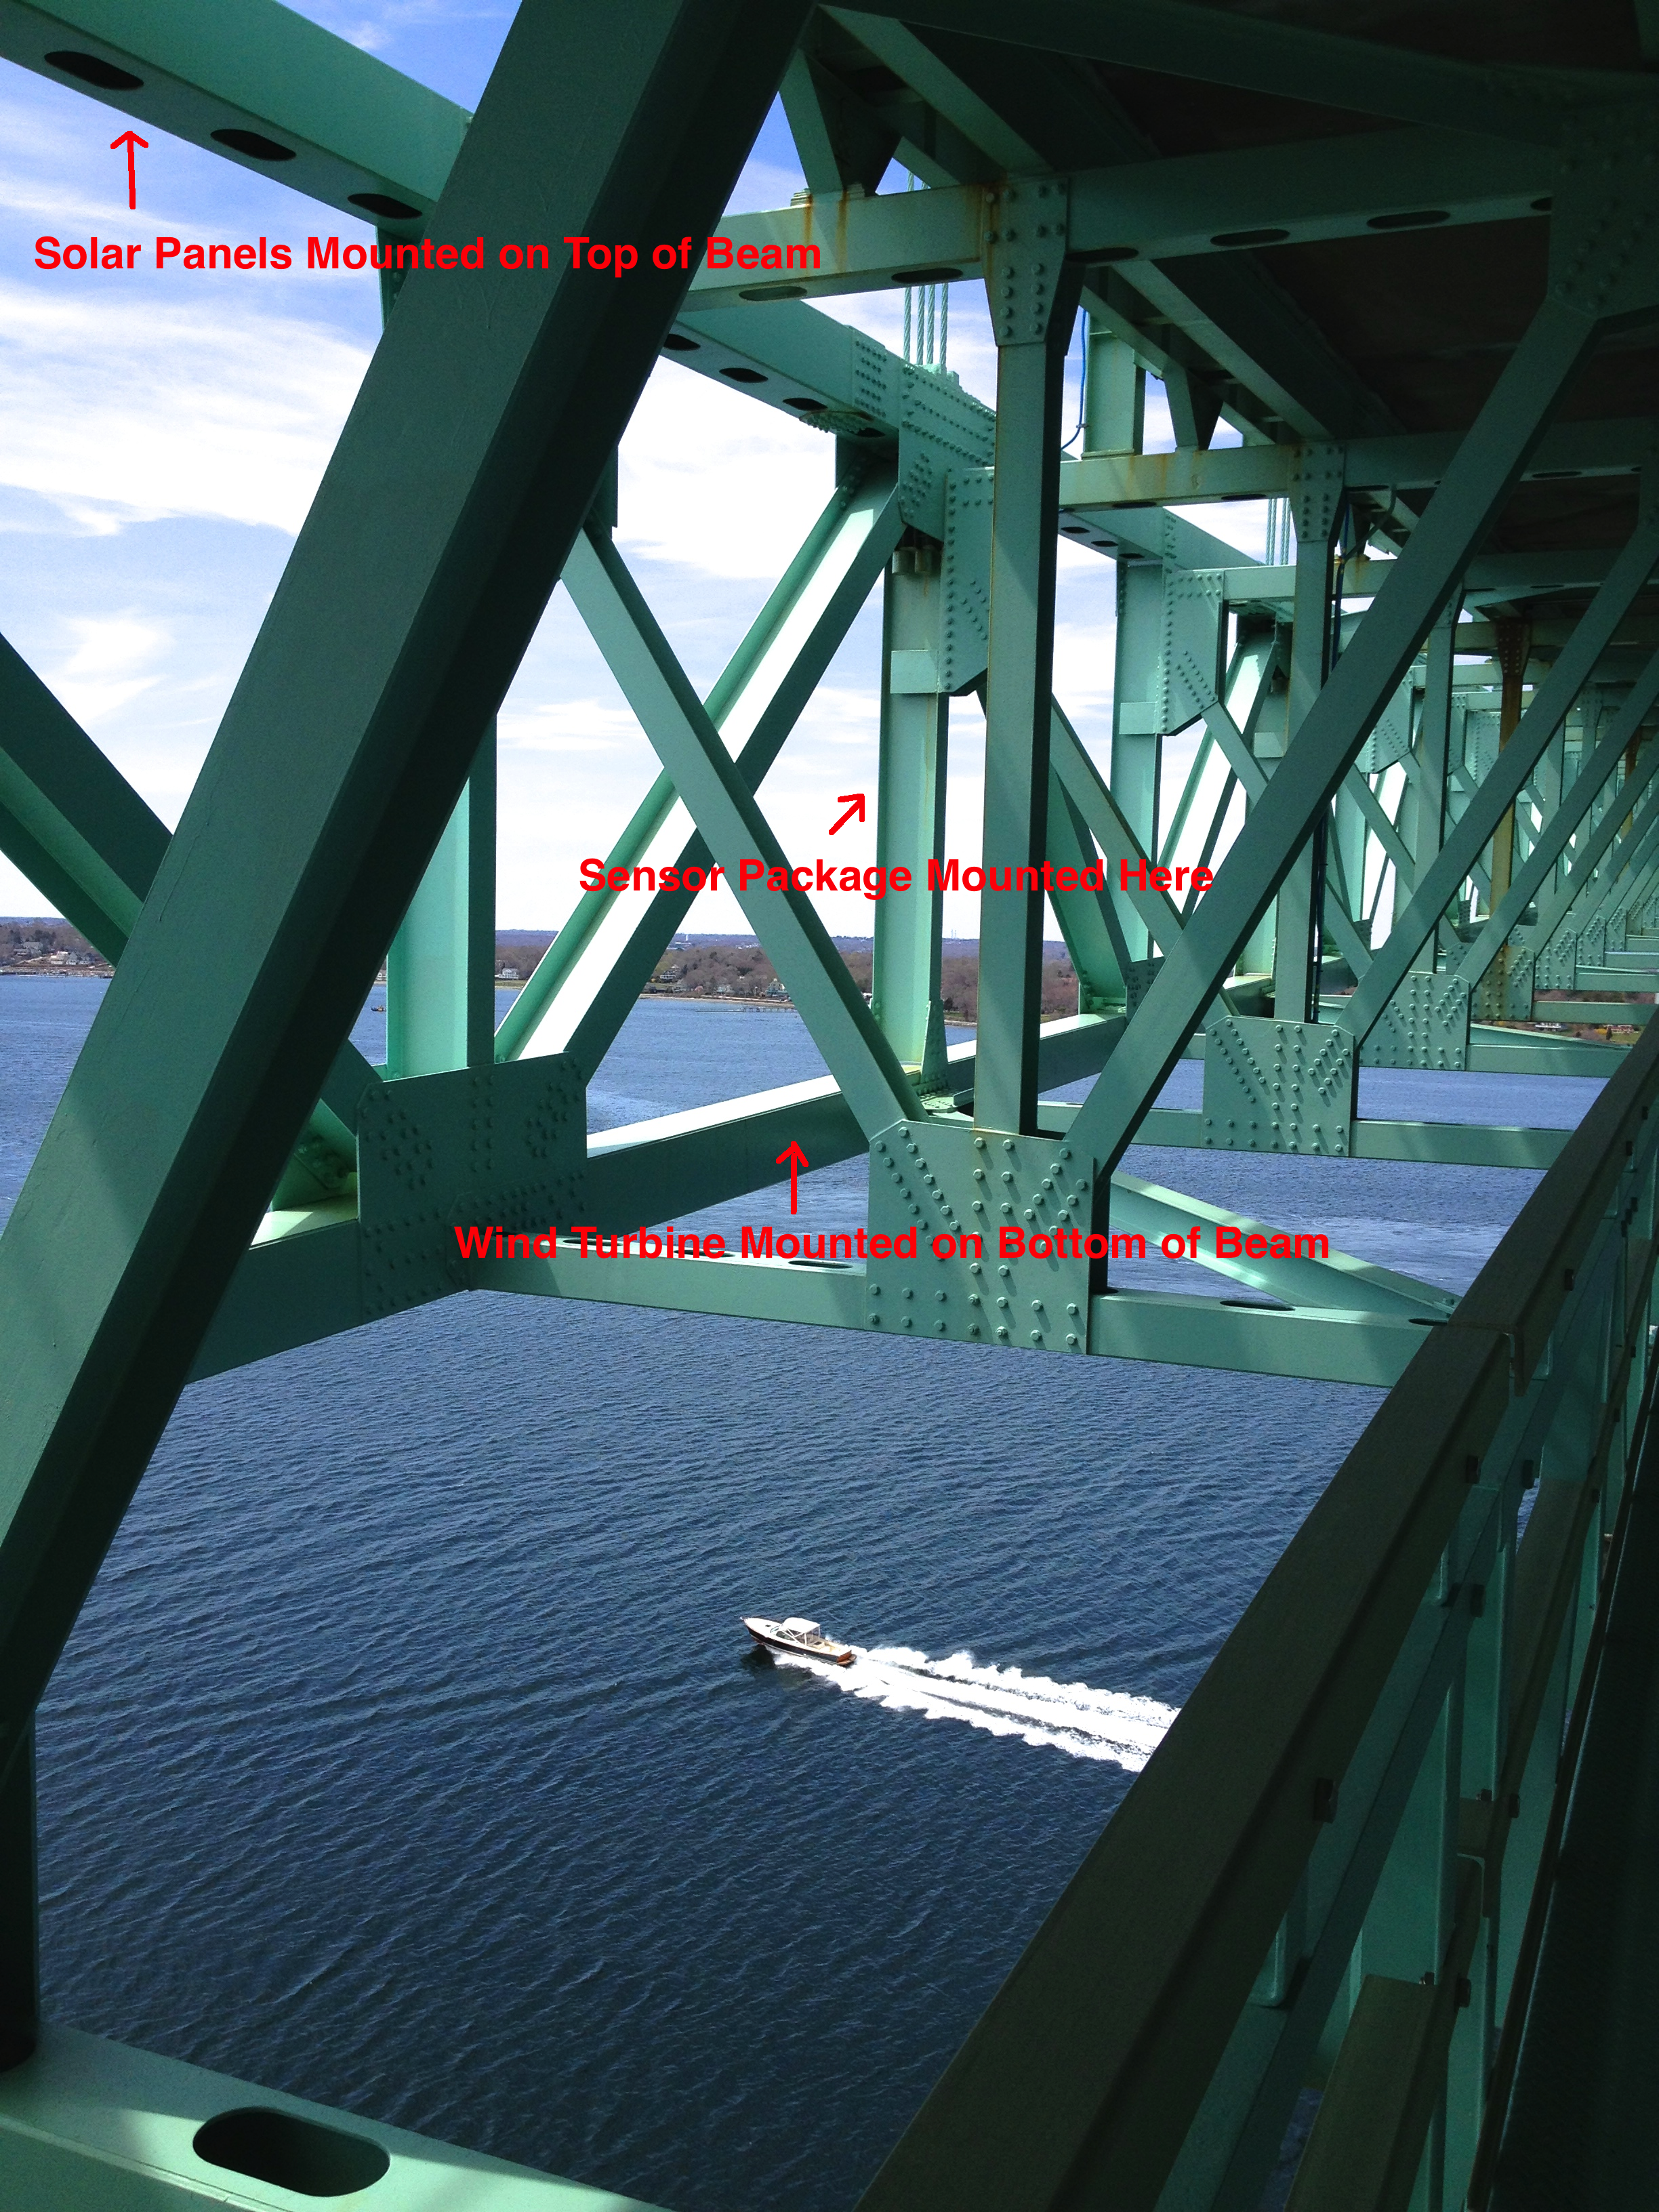
\includegraphics[width=0.3\textwidth]{Proposed_Package_Location.png}
\caption{Proposed Location for Sensor Package, Wind Turbine and Solar Panels.}
\label{fig:Proposed Package, Panels and Turbine Location}
\end{figure}




\section{Appendix Case Comparison}
\begin{table}[h]
\begin{tabular}{lllllllp{3cm}}
Company   & Case Model   & Length & Width & Height & Weight & Cost   & Thermal Conductivity Coefficient (W/m*$^{\circ}$C) \\
Pelican   & 1300      & 9.17  & 7.00 & 6.12  & 3.09  & \$55.65 & 0.1-0.22                       \\
~      & 1400      & 11.81 & 8.87 & 5.18  & 3.97  & \$81.58 & 0.1-0.22                       \\
~      & 1450      & 14.62 & 10.18 & 6   & 5.51  & \$103.73 & 0.1-0.22                       \\
~      & 1460      & 18.54 & 9.92 & 10.92 & 8.75  & \$180.59 & 0.1-0.22                       \\
Fibox    & PC MH 125 G  & 9.1  & 5.5  & 4.9  & NA   & NA    & 0.19                         \\
~      & PC 2828 18 G  & 10.9  & 10.9 & 7.1  & NA   & NA    & 0.19                         \\
~      & PC 175/150 XHG & 7.1  & 7.1  & 5.9  & NA   & NA    & 0.19                         \\
Nanuk    & 9.4      & 9.4  & 7.4  & 5.5  & 3.3  & \$38.95 & 0.1-0.22                       \\
~      & 915      & 13.8  & 9.3  & 6.2  & 4.4  & \$63.95 & 0.1-0.22                       \\
UW Kinetics & Ultra-case 613 & 13.4  & 8.9  & 5.6  & 4.5  & \$148.99 & 0.2                         \\
\end{tabular}
\end{table}
